\section{Recap}

\begin{frame}{Mathematical Model for the Sedimentation of Rod-Like Particles}
	\scriptsize
\text{Coupling of a kinetic Smoluchowski equation with Navier-Stokes equation}
\begin{align*}
\partial_t f+ \nabla_{\boldsymbol{x}} \cdot(\boldsymbol{u} f) & +\nabla_{\boldsymbol{n}} \cdot\left(P_{\boldsymbol{n}^{\perp}} \nabla_{\boldsymbol{x}} \boldsymbol{u} \boldsymbol{n} f\right)- \nabla_{\boldsymbol{x}} \cdot\left((I+\boldsymbol{n} \otimes \boldsymbol{n}) \boldsymbol{e_3} f\right) \\
	& =D_r \Delta_n f, \\
	\operatorname{Re}\left(\partial_t \boldsymbol{u}+\left(\boldsymbol{u} \cdot \nabla_{\boldsymbol{x}}\right) \boldsymbol{u}\right) & =\Delta_{\boldsymbol{x}} \boldsymbol{u}-\nabla_{\boldsymbol{x}} p-\delta \left(\int_{S^{d-1}} f d \boldsymbol{n} \right) \boldsymbol{e_3}, \\
	\nabla_{\boldsymbol{x}} \cdot \boldsymbol{u} & =0,
\end{align*}
where $f = f(\boldsymbol{x}, t, \boldsymbol{n})$ represents the particle distribution of rod-like particles as a function of time $t$, space $\boldsymbol{x} \in \mathbb{R}^3$ and orientation $\boldsymbol{n} \in  S^2$. 
$D_r, \delta$ and $Re$ are non-dimensional parameters.
\begin{beamercolorbox}[sep=1em,wd=\linewidth,right]{}
	\tiny{Helzel $\&$ Tzavaras, 2017}
\end{beamercolorbox}
\end{frame}

\begin{frame}{2D: Coupled System for Rectilinear Flow}
	\scriptsize
	We consider $\boldsymbol{u} = \left( 0, 0, w(x,y, t)\right)^T$, $f(x,y,t,\phi,\theta)$. We get
	\begin{equation}
		\begin{aligned}
			&\sin\theta \partial_{t}f(x,y,t,\phi, \theta)+ \textcolor{red}{\partial_x(\cos\phi \sin\theta \cos\theta f)} + \textcolor{red}{\partial_y(\sin \phi \sin \theta \cos \theta f)} \\
			&+ \textcolor{blue}{\partial_\theta\left(( w_x \sin^3 \theta \cos \phi + w_y\sin \phi \sin^3 \theta) f\right)}
			= \textcolor{blue}{D_{r}\left( \partial_\phi \left(\frac{1}{\sin \theta} \partial_\phi f \right)+ \partial_\theta (\sin \theta \partial_\theta f)\right)} \\
			&Re\partial_{t}w(x,y,t) = \partial_{xx}w + \partial_{yy}w + \delta\left(\bar{\rho}-\int_{0}^{2\pi} \int_{0}^{\pi} f \sin \theta d\theta d\phi \right).
		\end{aligned}
	\end{equation}
	\pause
	The system of hierarchy of moment equations is given as
	\begin{equation}
		\partial_t Q + \textcolor{red}{A  \partial_x Q}
		+ \textcolor{red}{B \partial_y Q} =  \textcolor{blue}{ D(w_x,w_y)Q+ D_rEQ},
	\end{equation}
    where $Q=(c^0_0(x,t), c^{-2}_2(x,t), \ldots, c^{2N}_{2N}(x,t))^T$ represents the vector of the moments and \\
    \vspace{2mm}
    $A,B,D,E \in \mathbb{R}^{(N+1)(2N+1)x(N+1)(2N+1)}$.
\end{frame}


\begin{frame}
	\scriptsize
	\begin{figure}[H]
		\centering
		\begin{minipage}{0.4\textwidth}
			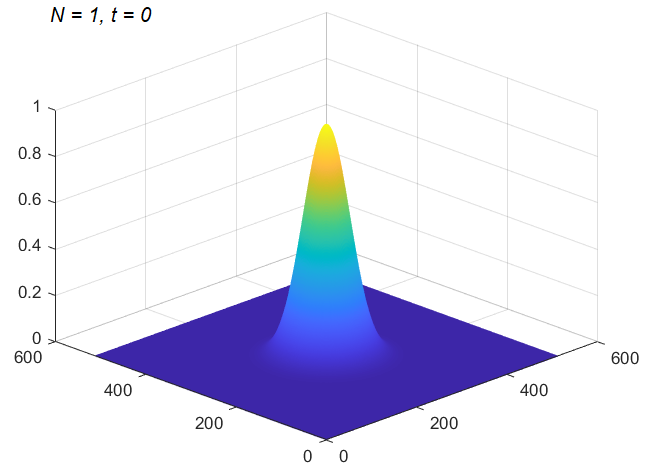
\includegraphics[scale=0.3]{Bilder_wxwy/t=0_wxwy=1_wxwy=-1}
		\end{minipage}
		\hfill 
		\begin{minipage}{0.4\textwidth}
			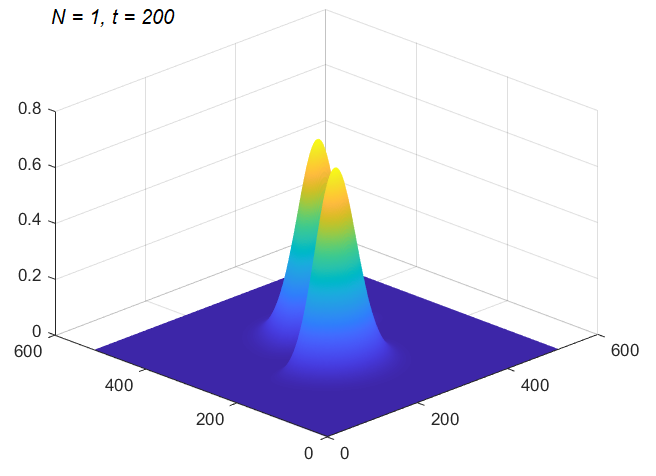
\includegraphics[scale=0.3]{Bilder_wxwy/t=200_wxwy=1_wxwy=-1}
		\end{minipage}
		\caption{Numerical results for $c^0_0$ at different times using $D_r=1$ and $w_x=w_y=1$ for $x<50$ and $w_x=w_y=-1$ otherwise. A cluster with higher particle density splits into two, each moving in opposite directions.}
		
	\begin{minipage}{0.4\textwidth}
		\centering
		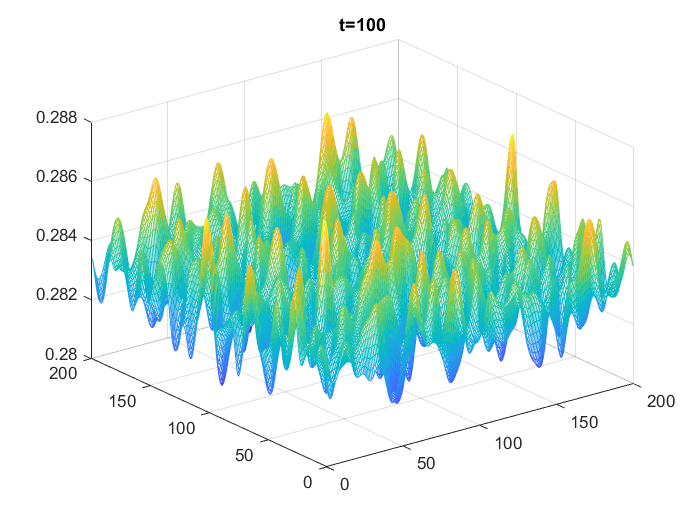
\includegraphics[scale=0.25]{Bilder_wxwy/14th_t=100_mx=my=200_random_Dr=1_(1.d0+(1.d-2rand(0)-5.d-4))Divide(2.d0dsqrt(pi))}
		\end{minipage}
		\hfill 
		\begin{minipage}{0.4\textwidth}
			\centering
			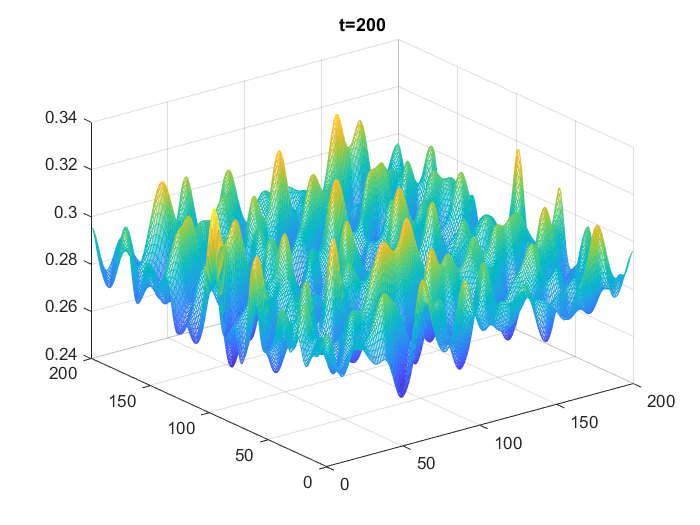
\includegraphics[scale=0.25]{Bilder_wxwy/14th_t=200_mx=my=200_random_Dr=1_(1.d0+(1.d-2rand(0)-5.d-4))Divide(2.d0dsqrt(pi))}
		\end{minipage}
		\caption{Solution structure of \(c^0_0\) with \(N = 7\).}
	\end{figure}
\end{frame}



%----------------------------------------------------------
%----------------------------------------------------------

\begin{frame}{Status of Project}
	\scriptsize
	\begin{block}{So far...}
		\begin{itemize}
		   \item <1-> Derive and approximate hierarchies of moment equations for the coupled kinetic-fluid model with \textcolor{cyan}{$f$ on $S^2$}
		   \begin{itemize}
			  \item  1D Shear Flow
		  	  \item  2D Rectilinear Flow
		   \end{itemize}
		\end{itemize}
	\end{block}
	\begin{block}{Now}
		\begin{itemize}
			\item <2-> Extension to the 3D case: moment equations for the coupled kinetic–fluid model with \textcolor{cyan}{$f$ on $S^2$}
		\end{itemize}
	\end{block}
\end{frame}





